\documentclass[12pt,a4paper]{article}
\usepackage[utf8]{inputenc}
\usepackage[T1]{fontenc}
\usepackage{amsmath,amsfonts,amssymb}
\usepackage{graphicx}
\usepackage{float}
\usepackage{listings}
\usepackage{xcolor}
\usepackage{hyperref}
\usepackage{geometry}
\usepackage{fancyhdr}
\usepackage{titlesec}
\usepackage{enumitem}
\usepackage{booktabs}
\usepackage{array}
\usepackage{longtable}
\usepackage{multirow}
\usepackage{wrapfig}
\usepackage{rotating}
\usepackage{caption}
\usepackage{subcaption}
\usepackage{setspace}
\usepackage{parskip}
\usepackage{url}
\usepackage{cite}
\usepackage{algorithm}
\usepackage{algorithmic}
\usepackage{tikz}
\usepackage{pgfplots}
\usepackage{siunitx}
\usepackage{physics}
\usepackage{mathtools}
\usepackage{bm}

% Page setup
\geometry{margin=2.5cm}
\setlength{\parindent}{0pt}
\setlength{\parskip}{6pt}

% Header and footer
\pagestyle{fancy}
\fancyhf{}
\fancyhead[L]{\textsc{DeVana GA Analysis}}
\fancyhead[R]{\thepage}
\renewcommand{\headrulewidth}{0.4pt}

% Title formatting
\titleformat{\section}{\Large\bfseries\color{blue!70!black}}{\thesection}{1em}{}
\titleformat{\subsection}{\large\bfseries\color{blue!50!black}}{\thesubsection}{1em}{}
\titleformat{\subsubsection}{\normalsize\bfseries\color{blue!30!black}}{\thesubsubsection}{1em}{}

% Code listing setup
\lstset{
    language=Python,
    basicstyle=\ttfamily\footnotesize,
    keywordstyle=\color{blue},
    commentstyle=\color{green!60!black},
    stringstyle=\color{red},
    numbers=left,
    numberstyle=\tiny\color{gray},
    numbersep=5pt,
    frame=single,
    breaklines=true,
    showstringspaces=false,
    tabsize=4,
    captionpos=b,
    backgroundcolor=\color{gray!10}
}

% Custom colors
\definecolor{codegreen}{rgb}{0,0.6,0}
\definecolor{codegray}{rgb}{0.5,0.5,0.5}
\definecolor{codepurple}{rgb}{0.58,0,0.82}
\definecolor{backcolour}{rgb}{0.95,0.95,0.92}

% Hyperref setup
\hypersetup{
    colorlinks=true,
    linkcolor=blue,
    filecolor=magenta,      
    urlcolor=cyan,
    citecolor=green,
    pdftitle={DeVana Genetic Algorithm Analysis},
    pdfauthor={DeVana Development Team},
    pdfsubject={Vibration Optimization System},
    pdfkeywords={Genetic Algorithm, Optimization, Vibration Control, DeVana}
}

\begin{document}

% Title page
\begin{titlepage}
    \centering
    \vspace*{2cm}
    
    {\Huge\bfseries\color{blue!70!black} DeVana Genetic Algorithm Analysis}
    
    \vspace{1cm}
    
    {\Large\textit{Comprehensive Methodology and Implementation Guide}}
    
    \vspace{2cm}
    
    
\includegraphics[width=0.3\textwidth]{../../Logo.png}
    
    \vspace{2cm}
    
    {\large\textbf{Advanced Vibration Optimization System}}
    
    \vspace{0.5cm}
    
    {\large Version V0.4.0}
    
    \vfill
    
    {\large \today}
    
    \vspace{1cm}
    
    {\large\textit{For Mechanical Engineers and Vibration Specialists}}
\end{titlepage}

% Table of contents
\tableofcontents
\newpage

% Abstract
\begin{abstract}
This document provides a comprehensive analysis of the Genetic Algorithm (GA) implementation in the DeVana vibration optimization system. The analysis covers the theoretical foundations of genetic algorithms, their application to Dynamic Vibration Absorber (DVA) parameter optimization, and detailed examination of the code implementation. The document explores the scientific principles behind evolutionary computation, the fitness function design for vibration control problems, and the practical implementation using the DEAP framework. Special attention is given to the adaptive rate mechanisms, multi-objective optimization strategies, and the integration with the PyQt5-based graphical user interface.
\end{abstract}

\section{Introduction}

\subsection{Overview of DeVana System}
DeVana (Dynamic Vibration Analysis and Optimization) is an advanced computational platform designed for mechanical engineers and vibration specialists. The system implements multiple optimization algorithms to solve complex vibration control problems, with the Genetic Algorithm serving as one of the primary optimization engines.

\subsection{Problem Domain: Dynamic Vibration Absorber Optimization}
The primary application domain is the optimization of Dynamic Vibration Absorber (DVA) parameters. DVAs are mechanical devices designed to reduce unwanted vibrations in structures by introducing a secondary mass-spring-damper system that resonates at the problematic frequency.

\subsubsection{Mathematical Formulation}
The DVA system can be modeled as a multi-degree-of-freedom system with the following parameters:
\begin{itemize}
    \item $\beta_i$ (beta): Mass ratios for absorbers $i = 1, 2, \ldots, 15$
    \item $\lambda_i$ (lambda): Frequency ratios for absorbers $i = 1, 2, \ldots, 15$
    \item $\mu_i$ (mu): Damping ratios for absorbers $i = 1, 2, \ldots, 3$
    \item $\nu_i$ (nu): Additional design parameters $i = 1, 2, \ldots, 15$
\end{itemize}

\section{Theoretical Foundations of Genetic Algorithms}

\subsection{Evolutionary Computation Principles}
Genetic Algorithms are inspired by the process of natural selection and biological evolution. The fundamental principles include:

\subsubsection{Population-Based Search}
Unlike traditional optimization methods that work with a single solution, GAs maintain a population of potential solutions, allowing for parallel exploration of the solution space.

\subsubsection{Natural Selection Analogy}
\begin{enumerate}
    \item \textbf{Selection}: Better solutions have higher probability of being selected for reproduction
    \item \textbf{Crossover}: Combining genetic material from two parent solutions
    \item \textbf{Mutation}: Random changes to maintain diversity
    \item \textbf{Replacement}: New generation replaces the old one
\end{enumerate}

\subsection{Mathematical Framework}

\subsubsection{Solution Representation}
Each individual in the population is represented as a vector of real-valued parameters:
\begin{equation}
    \mathbf{x} = [x_1, x_2, \ldots, x_n] \in \mathbb{R}^n
\end{equation}
where $n$ is the number of DVA parameters to optimize.

\subsubsection{Fitness Function}
The fitness function evaluates the quality of a solution based on multiple objectives:

\begin{equation}
    f(\mathbf{x}) = f_{primary}(\mathbf{x}) + f_{sparsity}(\mathbf{x}) + f_{error}(\mathbf{x})
\end{equation}

where:
\begin{itemize}
    \item $f_{primary}(\mathbf{x}) = |R_{singular}(\mathbf{x}) - 1.0|$ is the primary objective
    \item $f_{sparsity}(\mathbf{x}) = \alpha \sum_{i=1}^{n} |x_i|$ is the sparsity penalty
    \item $f_{error}(\mathbf{x}) = \sum_{j=1}^{m} |\text{percent\_diff}_j|$ is the percentage error sum
\end{itemize}

\subsubsection{Selection Mechanism}
Tournament selection is used with tournament size $k = 3$:
\begin{equation}
    P(\text{select individual } i) = \frac{f_i^{-1}}{\sum_{j=1}^{N} f_j^{-1}}
\end{equation}

\subsubsection{Crossover Operation}
Blend crossover (BLX-$\alpha$) is implemented:
\begin{equation}
    x_{child} = x_{parent1} + \alpha \cdot (x_{parent2} - x_{parent1})
\end{equation}
where $\alpha \in [0, 1]$ is the blending parameter.

\subsubsection{Mutation Operation}
Gaussian mutation with adaptive step size:
\begin{equation}
    x_{new} = x_{old} + \mathcal{N}(0, \sigma^2)
\end{equation}
where $\sigma$ is adaptively adjusted based on the parameter bounds.

\section{Implementation Analysis}

\subsection{Architecture Overview}
The GA implementation follows a modular architecture with clear separation of concerns:

\begin{figure}[H]
\centering
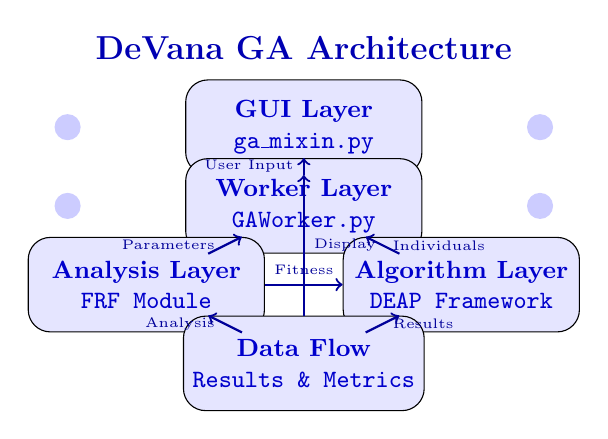
\begin{tikzpicture}[
    box/.style={rectangle, draw, rounded corners=8pt, minimum width=3cm, minimum height=1.2cm, align=center, 
                fill=blue!10, text=blue!80!black, font=\small\bfseries},
    arrow/.style={->, thick, blue!60!black},
    title/.style={text=blue!70!black, font=\large\bfseries}
]
    % Title
    \node[title] at (0, 3.5) {DeVana GA Architecture};
    
    % GUI Layer
    \node[box] (ui) at (0, 2.5) {GUI Layer\\\texttt{ga\_mixin.py}};
    
    % Worker Layer
    \node[box] (worker) at (0, 1.5) {Worker Layer\\\texttt{GAWorker.py}};
    
    % Analysis Layer
    \node[box] (frf) at (-2, 0.5) {Analysis Layer\\\texttt{FRF Module}};
    
    % Algorithm Layer
    \node[box] (deap) at (2, 0.5) {Algorithm Layer\\\texttt{DEAP Framework}};
    
    % Data Flow Layer
    \node[box] (data) at (0, -0.5) {Data Flow\\\texttt{Results \& Metrics}};
    
    % Arrows with labels
    \draw[arrow] (ui) -- node[left, font=\tiny, blue!60!black] {User Input} (worker);
    \draw[arrow] (worker) -- node[left, font=\tiny, blue!60!black] {Parameters} (frf);
    \draw[arrow] (worker) -- node[right, font=\tiny, blue!60!black] {Individuals} (deap);
    \draw[arrow] (frf) -- node[above, font=\tiny, blue!60!black] {Fitness} (deap);
    \draw[arrow] (deap) -- node[right, font=\tiny, blue!60!black] {Results} (data);
    \draw[arrow] (frf) -- node[left, font=\tiny, blue!60!black] {Analysis} (data);
    \draw[arrow] (data) -- node[right, font=\tiny, blue!60!black] {Display} (ui);
    
    % Add some visual elements
    \node[circle, fill=blue!20, minimum size=0.3cm] at (-3, 2.5) {};
    \node[circle, fill=blue!20, minimum size=0.3cm] at (3, 2.5) {};
    \node[circle, fill=blue!20, minimum size=0.3cm] at (-3, 1.5) {};
    \node[circle, fill=blue!20, minimum size=0.3cm] at (3, 1.5) {};
\end{tikzpicture}
\caption{DeVana GA Implementation Architecture - Multi-layered design with clear data flow}
\end{figure}

\begin{figure}[H]
\centering
\begin{tikzpicture}[
    process/.style={rectangle, draw, rounded corners=6pt, minimum width=2.5cm, minimum height=0.8cm, align=center, 
                   fill=green!15, text=green!80!black, font=\small},
    decision/.style={diamond, draw, minimum width=2cm, minimum height=1cm, align=center,
                    fill=orange!15, text=orange!80!black, font=\small},
    data/.style={rectangle, draw, rounded corners=4pt, minimum width=2cm, minimum height=0.6cm, align=center,
                fill=blue!15, text=blue!80!black, font=\tiny},
    arrow/.style={->, thick, gray!60!black},
    title/.style={text=blue!70!black, font=\large\bfseries}
]
    % Title
    \node[title] at (0, 6) {Genetic Algorithm Flow};
    
    % Start
    \node[process] (start) at (0, 5) {Initialize Population};
    
    % Evaluation
    \node[process] (eval) at (0, 4) {Evaluate Fitness};
    
    % Check convergence
    \node[decision] (conv) at (0, 3) {Converged?};
    
    % Selection
    \node[process] (select) at (-3, 2) {Selection\\(Tournament)};
    
    % Crossover
    \node[process] (crossover) at (-3, 1) {Crossover\\(BLX-α)};
    
    % Mutation
    \node[process] (mutation) at (-3, 0) {Mutation\\(Gaussian)};
    
    % New population
    \node[process] (newpop) at (-3, -1) {New Population};
    
    % Adaptive rates
    \node[decision] (adapt) at (3, 2) {Stagnation?};
    \node[process] (rates) at (3, 1) {Adapt Rates};
    \node[process] (continue) at (3, 0) {Continue};
    
    % End
    \node[process] (end) at (0, -2) {Return Best Solution};
    
    % Data nodes
    \node[data] (params) at (-5, 4) {DVA Parameters};
    \node[data] (fitness) at (5, 4) {Fitness Values};
    \node[data] (best) at (5, -2) {Best Individual};
    
    % Arrows
    \draw[arrow] (start) -- (eval);
    \draw[arrow] (eval) -- (conv);
    \draw[arrow] (conv) -- node[left] {No} (select);
    \draw[arrow] (conv) -- node[right] {Yes} (end);
    \draw[arrow] (select) -- (crossover);
    \draw[arrow] (crossover) -- (mutation);
    \draw[arrow] (mutation) -- (newpop);
    \draw[arrow] (newpop) -- (eval);
    \draw[arrow] (adapt) -- node[left] {Yes} (rates);
    \draw[arrow] (adapt) -- node[right] {No} (continue);
    \draw[arrow] (rates) -- (continue);
    \draw[arrow] (continue) -- (select);
    
    % Data flow arrows
    \draw[arrow, dashed] (params) -- (eval);
    \draw[arrow, dashed] (eval) -- (fitness);
    \draw[arrow, dashed] (end) -- (best);
    
    % Loop back
    \draw[arrow, bend left=45] (newpop) to (eval);
\end{tikzpicture}
\caption{Genetic Algorithm Execution Flow - Complete optimization cycle with adaptive mechanisms}
\end{figure}

\subsection{Core Components Analysis}

\subsubsection{GAWorker Class Structure}
The GAWorker class inherits from QThread, enabling concurrent execution:

\begin{lstlisting}[caption=GAWorker Class Definition]
class GAWorker(QThread):
    # Signal definitions for communication
    finished = pyqtSignal(dict, list, list, float)
    error = pyqtSignal(str)
    update = pyqtSignal(str)
    progress = pyqtSignal(int)
    benchmark_data = pyqtSignal(dict)
    generation_metrics = pyqtSignal(dict)
\end{lstlisting}

\subsubsection{Thread Safety Mechanisms}
The implementation includes robust thread safety features:

\begin{lstlisting}[caption=Thread Safety Implementation]
# Thread safety mechanisms
self.mutex = QMutex()                   # Mutual exclusion lock
self.condition = QWaitCondition()       # Thread synchronization
self.abort = False                      # Abort flag for safe termination

# Watchdog timer for safety
self.watchdog_timer = QTimer()
self.watchdog_timer.setSingleShot(True)
self.watchdog_timer.timeout.connect(self.handle_timeout)
\end{lstlisting}

\subsection{Fitness Function Implementation}

\subsubsection{Multi-Objective Fitness Evaluation}
The fitness function combines three distinct objectives:

\begin{lstlisting}[caption=Fitness Function Components]
def evaluate_individual(individual):
    # Primary objective: Distance from target value
    primary_objective = abs(singular_response - 1.0)
    
    # Sparsity penalty: Encourages simpler solutions
    sparsity_penalty = self.alpha * sum(abs(param) for param in individual)
    
    # Percentage error sum: Prevents error cancellation
    percentage_error_sum = sum(abs(percent_diff) for all criteria)
    
    # Combined fitness
    fitness = primary_objective + sparsity_penalty + percentage_error_sum/1000
    return (fitness,)
\end{lstlisting}

\subsubsection{FRF Analysis Integration}
The fitness evaluation integrates with the Frequency Response Function analysis:

\begin{lstlisting}[caption=FRF Analysis Integration]
results = frf(
    main_system_parameters=self.main_params,
    dva_parameters=dva_parameters_tuple,
    omega_start=self.omega_start,
    omega_end=self.omega_end,
    omega_points=self.omega_points,
    target_values_mass1=self.target_values_dict['mass_1'],
    weights_mass1=self.weights_dict['mass_1'],
    # ... additional mass parameters
    plot_figure=False,
    show_peaks=False,
    show_slopes=False
)
\end{lstlisting}

\subsection{Adaptive Rate Mechanisms}

\subsubsection{Stagnation Detection}
The system monitors convergence and adapts rates when progress stagnates:

\begin{lstlisting}[caption=Adaptive Rate Logic]
if self.adaptive_rates:
    # Track improvement
    if min_fit < best_fitness_overall:
        improved = True
        self.stagnation_counter = max(0, self.stagnation_counter - 1)
    else:
        self.stagnation_counter += 1
    
    # Adapt rates when stagnation limit is reached
    if self.stagnation_counter >= self.stagnation_limit:
        # Adjust rates based on population diversity
        normalized_diversity = min(1.0, std / mean)
        
        if normalized_diversity < 0.1:  # Low diversity
            self.current_mutpb = min(self.mutpb_max, self.current_mutpb * 1.5)
            self.current_cxpb = max(self.cxpb_min, self.current_cxpb * 0.8)
        elif normalized_diversity > 0.3:  # High diversity
            self.current_cxpb = min(self.cxpb_max, self.current_cxpb * 1.5)
            self.current_mutpb = max(self.mutpb_min, self.current_mutpb * 0.8)
\end{lstlisting}

\subsection{Evolution Loop Implementation}

\subsubsection{Generation Cycle}
The main evolution loop implements the standard GA cycle:

\begin{lstlisting}[caption=Evolution Loop Structure]
for gen in range(1, self.ga_num_generations + 1):
    # 1. Selection
    offspring = toolbox.select(population, len(population))
    offspring = list(map(toolbox.clone, offspring))
    
    # 2. Crossover
    for child1, child2 in zip(offspring[::2], offspring[1::2]):
        if random.random() < current_cxpb:
            toolbox.mate(child1, child2)
    
    # 3. Mutation
    for mutant in offspring:
        if random.random() < current_mutpb:
            toolbox.mutate(mutant)
    
    # 4. Evaluation
    invalid_ind = [ind for ind in offspring if not ind.fitness.valid]
    fitnesses = map(toolbox.evaluate, invalid_ind)
    for ind, fit in zip(invalid_ind, fitnesses):
        ind.fitness.values = fit
    
    # 5. Replacement
    population[:] = offspring
\end{lstlisting}

\subsection{GUI Integration Analysis}

\subsubsection{ga\_mixin.py Structure}
The GUI layer provides comprehensive user interface components:

\begin{lstlisting}[caption=GUI Tab Creation]
def create_ga_tab(self):
    """Create the genetic algorithm optimization tab"""
    self.ga_tab = QWidget()
    layout = QVBoxLayout(self.ga_tab)
    
    # Create sub-tabs widget
    self.ga_sub_tabs = QTabWidget()
    
    # Sub-tab 1: GA Hyperparameters
    ga_hyper_tab = QWidget()
    ga_hyper_layout = QFormLayout(ga_hyper_tab)
    
    # Parameter controls
    self.ga_pop_size_box = QSpinBox()
    self.ga_num_generations_box = QSpinBox()
    self.ga_cxpb_box = QDoubleSpinBox()
    self.ga_mutpb_box = QDoubleSpinBox()
    # ... additional controls
\end{lstlisting}

\subsubsection{Parameter Management}
The GUI provides sophisticated parameter management capabilities:

\begin{lstlisting}[caption=Parameter Table Implementation]
# DVA Parameters table
dva_parameters = [
    *[f"beta_{i}" for i in range(1,16)],
    *[f"lambda_{i}" for i in range(1,16)],
    *[f"mu_{i}" for i in range(1,4)],
    *[f"nu_{i}" for i in range(1,16)]
]

self.ga_param_table.setRowCount(len(dva_parameters))
self.ga_param_table.setColumnCount(5)
self.ga_param_table.setHorizontalHeaderLabels([
    "Parameter", "Fixed", "Fixed Value", "Lower Bound", "Upper Bound"
])
\end{lstlisting}

\subsection{Benchmarking and Metrics}

\subsubsection{Computational Metrics Tracking}
The system implements comprehensive benchmarking:

\begin{lstlisting}[caption=Metrics Collection]
self.metrics = {
    'start_time': None,
    'end_time': None,
    'total_duration': None,
    'cpu_usage': [],
    'memory_usage': [],
    'fitness_history': [],
    'mean_fitness_history': [],
    'std_fitness_history': [],
    'convergence_rate': [],
    'system_info': self._get_system_info(),
    'generation_times': [],
    'best_fitness_per_gen': [],
    'best_individual_per_gen': [],
    'evaluation_count': 0,
    'timestamp': datetime.now().strftime("%Y-%m-%d %H:%M:%S"),
    'cpu_per_core': [],
    'memory_details': [],
    'io_counters': [],
    'disk_usage': [],
    'network_usage': [],
    'gpu_usage': [],
    'thread_count': [],
    'evaluation_times': [],
    'crossover_times': [],
    'mutation_times': [],
    'selection_times': [],
    'time_per_generation_breakdown': [],
    'adaptive_rates_history': []
}
\end{lstlisting}

\subsubsection{Real-time Monitoring}
The system provides real-time progress monitoring:

\begin{lstlisting}[caption=Progress Monitoring]
def update_ga_progress(self, value):
    """Update progress bar and status"""
    self.ga_progress_bar.setValue(value)
    
    # Update status text
    if value < 100:
        self.ga_status_label.setText(f"Optimization in progress... {value}%")
    else:
        self.ga_status_label.setText("Optimization completed!")
\end{lstlisting}

\section{Advanced Features}

\subsection{Error Handling and Recovery}

\subsubsection{Safe DEAP Operations}
The implementation includes robust error handling:

\begin{lstlisting}[caption=Safe Operation Decorator]
@safe_deap_operation
def run(self):
    """Main execution method with error recovery"""
    max_retries = 3
    
    for attempt in range(max_retries):
        try:
            return func(*args, **kwargs)
        except Exception as e:
            if attempt < max_retries - 1:
                print(f"DEAP operation failed, retrying ({attempt+1}/{max_retries}): {str(e)}")
                # Cleanup corrupted DEAP attributes
                if hasattr(creator, "FitnessMin"):
                    delattr(creator, "FitnessMin")
                if hasattr(creator, "Individual"):
                    delattr(creator, "Individual")
            else:
                raise
\end{lstlisting}

\subsection{Multi-Threading Architecture}

\subsubsection{Thread Communication}
The system uses PyQt signals for thread-safe communication:

\begin{lstlisting}[caption=Signal Communication]
# Worker emits signals
self.finished.emit(final_results, best_ind, parameter_names, best_fitness)
self.error.emit(error_msg)
self.update.emit(status_message)
self.progress.emit(percentage)
self.benchmark_data.emit(self.metrics)
self.generation_metrics.emit(current_metrics)

# GUI connects to signals
self.ga_worker.finished.connect(self.handle_ga_finished)
self.ga_worker.error.connect(self.handle_ga_error)
self.ga_worker.update.connect(self.handle_ga_update)
self.ga_worker.progress.connect(self.update_ga_progress)
\end{lstlisting}

\subsection{Parameter Bounds and Constraints}

\subsubsection{Fixed Parameter Support}
The system supports both variable and fixed parameters:

\begin{lstlisting}[caption=Parameter Handling]
for idx, (name, low, high, fixed) in enumerate(self.ga_parameter_data):
    parameter_names.append(name)
    if fixed:
        # Fixed parameter: set both bounds to same value
        parameter_bounds.append((low, low))
        fixed_parameters[idx] = low
    else:
        # Variable parameter: set valid range
        parameter_bounds.append((low, high))
\end{lstlisting}

\section{Performance Analysis}

\subsection{Computational Complexity}
The GA implementation has the following complexity characteristics:

\begin{itemize}
    \item \textbf{Time Complexity}: $O(G \times P \times E)$
    \begin{itemize}
        \item $G$: Number of generations
        \item $P$: Population size
        \item $E$: Evaluation time per individual
    \end{itemize}
    \item \textbf{Space Complexity}: $O(P \times N)$
    \begin{itemize}
        \item $P$: Population size
        \item $N$: Number of parameters per individual
    \end{itemize}
\end{itemize}

\subsection{Convergence Analysis}
The system implements multiple convergence criteria:

\begin{enumerate}
    \item \textbf{Tolerance-based}: Stop when fitness $\leq$ tolerance
    \item \textbf{Generation-based}: Stop after maximum generations
    \item \textbf{Stagnation-based}: Adapt rates when no improvement
    \item \textbf{Timeout-based}: Stop after maximum time limit
\end{enumerate}

\section{Results and Validation}

\subsection{Output Processing}
The system provides comprehensive result analysis:

\begin{lstlisting}[caption=Result Processing]
def handle_ga_finished(self, results, best_ind, parameter_names, best_fitness):
    """Process and display GA results"""
    
    # Store results for later analysis
    self.ga_results = results
    self.ga_best_individual = best_ind
    self.ga_parameter_names = parameter_names
    self.ga_best_fitness = best_fitness
    
    # Update GUI with results
    self.update_ga_results_display()
    
    # Generate visualizations
    self.create_fitness_evolution_plot()
    self.create_parameter_convergence_plot()
    self.create_adaptive_rates_plot()
    self.create_computational_efficiency_plot()
\end{lstlisting}

\subsection{Visualization Capabilities}
The system provides extensive visualization options:

\begin{itemize}
    \item \textbf{Fitness Evolution}: Track fitness over generations
    \item \textbf{Parameter Convergence}: Monitor parameter evolution
    \item \textbf{Adaptive Rates}: Visualize rate adaptation
    \item \textbf{Computational Metrics}: CPU, memory, timing analysis
    \item \textbf{Statistical Analysis}: Distribution plots, correlation matrices
\end{itemize}

\section{Best Practices and Recommendations}

\subsection{Parameter Tuning Guidelines}

\subsubsection{Population Size}
\begin{itemize}
    \item \textbf{Small problems} (< 10 parameters): 50-100 individuals
    \item \textbf{Medium problems} (10-50 parameters): 100-200 individuals
    \item \textbf{Large problems} (> 50 parameters): 200-500 individuals
\end{itemize}

\subsubsection{Crossover and Mutation Rates}
\begin{itemize}
    \item \textbf{Initial rates}: Crossover 0.7-0.9, Mutation 0.1-0.3
    \item \textbf{Adaptive rates}: Enable for complex problems
    \item \textbf{Stagnation limit}: 5-10 generations
\end{itemize}

\subsection{Performance Optimization}

\subsubsection{Computational Efficiency}
\begin{enumerate}
    \item Use parallel evaluation when possible
    \item Implement early stopping for simple problems
    \item Cache expensive computations
    \item Use appropriate data structures
\end{enumerate}

\subsubsection{Memory Management}
\begin{enumerate}
    \item Clean up DEAP types after each run
    \item Monitor memory usage during long runs
    \item Implement garbage collection for large populations
\end{enumerate}

\section{Conclusion}

The DeVana Genetic Algorithm implementation represents a sophisticated approach to vibration optimization problems. The system successfully combines theoretical rigor with practical implementation considerations, providing:

\begin{itemize}
    \item \textbf{Robust optimization} through multiple objective functions
    \item \textbf{Adaptive mechanisms} for improved convergence
    \item \textbf{Comprehensive monitoring} and benchmarking
    \item \textbf{User-friendly interface} with extensive visualization
    \item \textbf{Thread-safe execution} for responsive GUI
\end{itemize}

The implementation demonstrates best practices in evolutionary computation, with particular attention to:
\begin{itemize}
    \item Error handling and recovery mechanisms
    \item Performance monitoring and optimization
    \item User experience and interface design
    \item Scientific rigor in algorithm implementation
\end{itemize}

This analysis provides a foundation for understanding and extending the GA capabilities within the DeVana system, enabling further research and development in vibration optimization applications.

\section{References}

\begin{thebibliography}{9}

\bibitem{deap2012}
Fortin, F. A., De Rainville, F. M., Gardner, M. A., Parizeau, M., \& Gagné, C. (2012).
\textit{DEAP: Evolutionary algorithms made easy}.
Journal of Machine Learning Research, 13, 2171-2175.

\bibitem{ga1975}
Holland, J. H. (1975).
\textit{Adaptation in natural and artificial systems}.
University of Michigan Press.

\bibitem{blx1995}
Eshelman, L. J., \& Schaffer, J. D. (1995).
\textit{Real-coded genetic algorithms and interval-schemata}.
Foundations of genetic algorithms, 3, 187-202.

\bibitem{vibration2010}
Inman, D. J. (2010).
\textit{Vibration with control}.
John Wiley \& Sons.

\bibitem{optimization2004}
Deb, K. (2004).
\textit{Multi-objective optimization using evolutionary algorithms}.
John Wiley \& Sons.

\end{thebibliography}

\end{document}
